\section{Resultados Obtenidos}

\begin{frame}{Resultados Obtenidos (1/7)}
\framesubtitle{Metodolog\'ia}

\framesubtitle{An\'alisis de Datos}
\vspace{-0.5em}
\begin{table}[H]
\centering
\scriptsize
\begin{tabular}{|p{0.9cm}|p{4.2cm}|p{2cm}|p{2cm}}
\hhline{---~}
M\'etrica  &   Descripci\'on & Valor  \\
\hhline{---~}
$M$ &   Resultado del test de memoria &  \textcolor{ForestGreen}{12,75 palabras} & \rdelim\}{1}{2cm}[Memoria del Usuario] \\
\rule{0pt}{4ex}$A$       &   Tasa de Acierto               &  \textcolor{ForestGreen}{83,70 \%} & \rdelim\}{3}{2cm}[\parbox{3cm-\tabcolsep-\widthof{$\Bigg]$}}{Correctitud de la Aplicaci\'on}] \\
 \rule{0pt}{4ex}$E_1$     & Tasa de Error de Comandos     &   \textcolor{Red}{16,30 \%}  \\
 \rule{0pt}{4ex}$E_2$     & Tasa de Error Humano          &   \textcolor{Red}{5,91 \%} &  \rdelim\}{3}{2cm}[Error Humano] \\
 \rule{0pt}{4ex}$E_3$     & Cantidad de Errores           &   \textcolor{Red}{11,83 errores}  \\
 \rule{0pt}{4ex}$T_{1+2}$ & Duraci\'on de Tareas Uno y Dos  & \textcolor{Red}{13,83 minutos}  & \rdelim\}{6}{2cm}[Eficiencia] \\
 \rule{0pt}{4ex}$T_{3+4}$ & Duraci\'on de Tareas Tres y Cuatro & \textcolor{Red}{18,35 minutos} \\
 \rule{0pt}{4ex}$C$       & Correctitud de la Tarea Cuatro  &    \textcolor{ForestGreen}{87,5 \%}  \\
 \rule{0pt}{4ex}$U$       & Cantidad de Comandos Utilizados &    \textcolor{ForestGreen}{40,67 comandos} \\
\cline{1-3} 
\end{tabular}
\end{table}

\textcolor{ForestGreen}{Mayor es mejor}

\textcolor{Red}{Menor es mejor}
\end{frame}

\begin{frame}{Resulados Obtenidos (2/7)}
\framesubtitle{Correlaci\'on}
\only<1>{\centering{Tasa de Acierto y Medidas del Error Humano}}
\only<2>{\begin{figure}[ht]
\centering
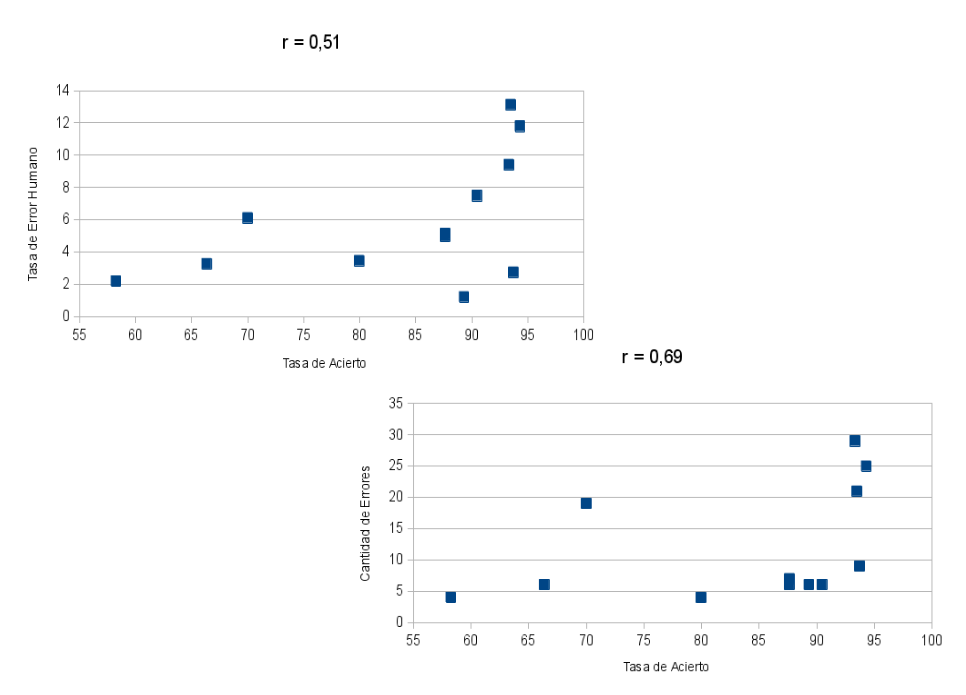
\includegraphics[width=1\linewidth]{./graphics/correlacion1.png}
\end{figure}}

\only<3>{Comandos utilizados, Medidas de Error Humano y Tasa de Acierto}
\only<4>{\begin{figure}[ht]
\centering
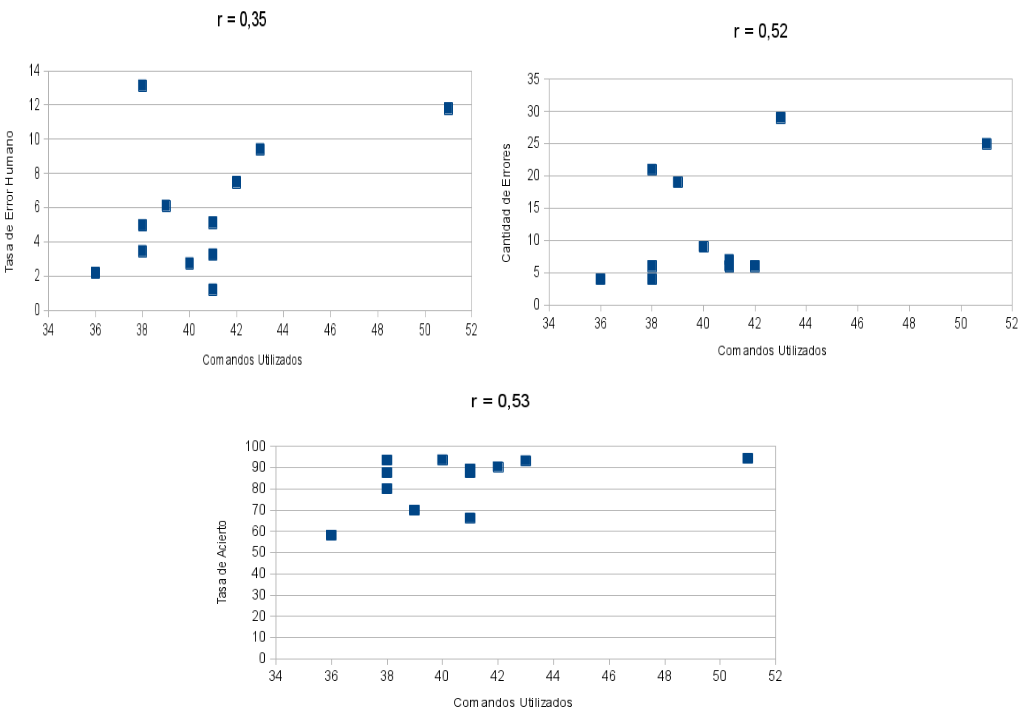
\includegraphics[width=1\linewidth]{./graphics/correlacion2.png}
\end{figure}}

\only<5>{Memoria del usuario, Tasa de Error Humano y Duraci\'on de las Tareas}
\only<6>{\begin{figure}[ht]
\centering
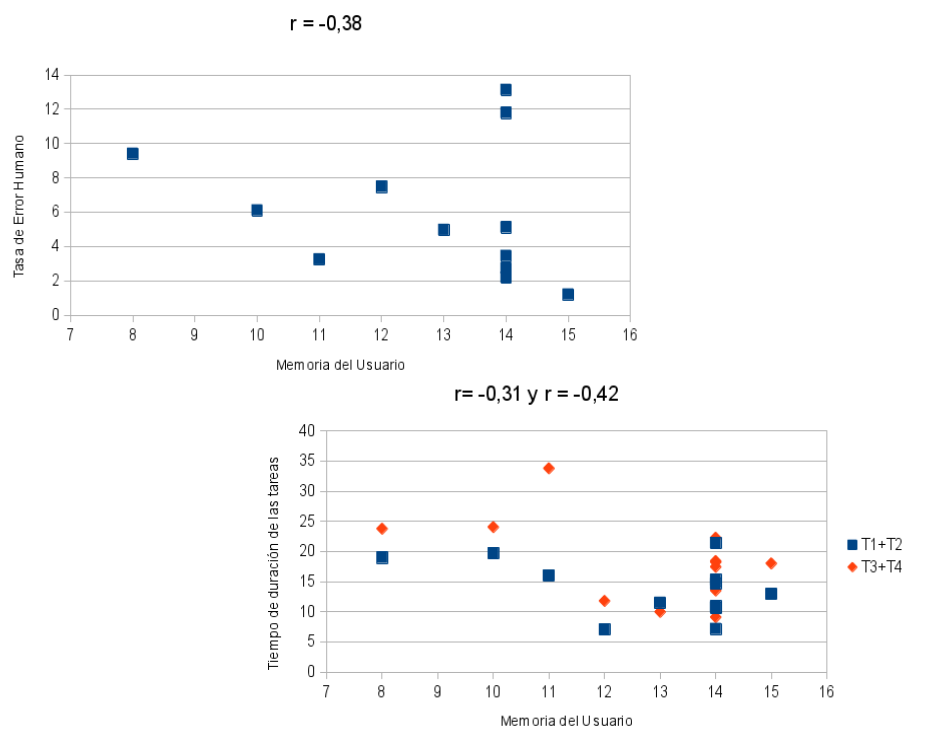
\includegraphics[width=0.9\linewidth]{./graphics/correlacion3.png}
\end{figure}}
\end{frame}


\begin{frame}{Resulados Obtenidos (3/7)}
\framesubtitle{Correlaci\'on}
\only<1>{\centering{Tasa de Acierto y Correctitud de la Tarea 4}}
\only<2>{\begin{figure}[ht]
\centering
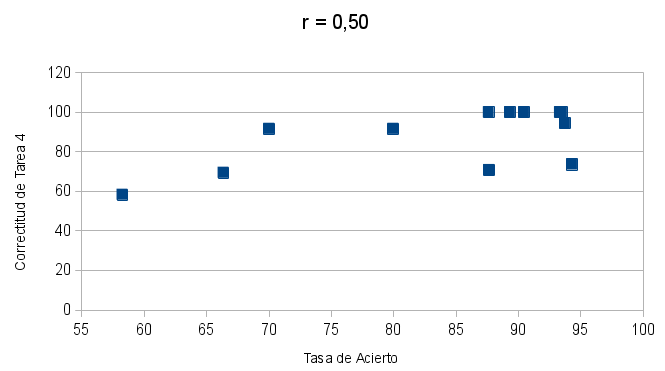
\includegraphics[width=0.9\linewidth]{./graphics/correlacion4.png}
\end{figure}}

\only<3>{\centering{Medidas de Error y Duraci\'on de las Tareas}}
\only<4>{\begin{figure}[ht]
\centering
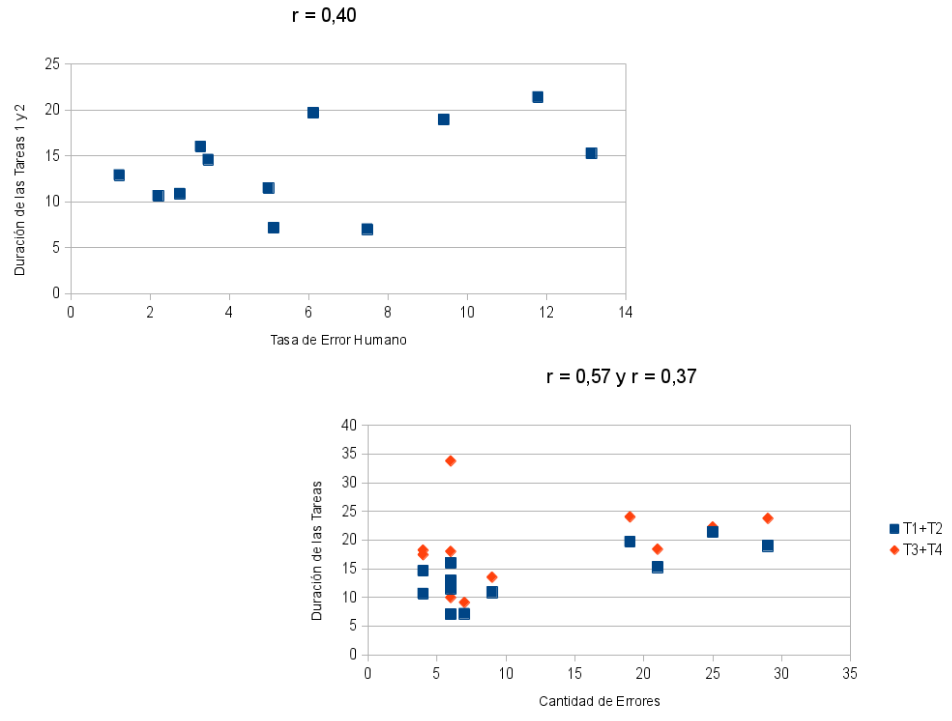
\includegraphics[width=0.9\linewidth]{./graphics/correlacion5.png}
\end{figure}}
\end{frame}

\begin{frame}{Resultados Obtenidos (4/7)}
\framesubtitle{An\'alisis del Error Humano}

\only<1>{\begin{figure}[ht]
\centering
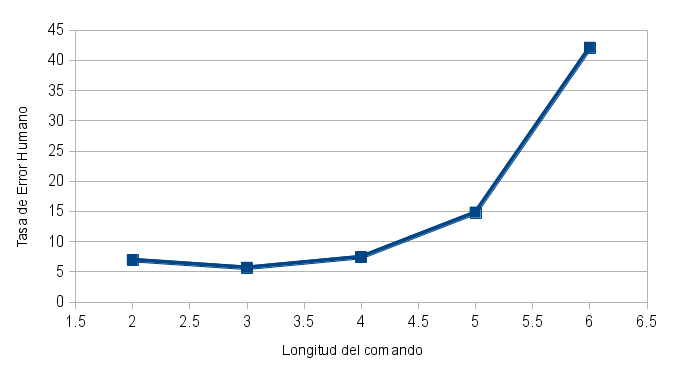
\includegraphics[width=0.9\linewidth]{./graphics/longitud-error.png}
\caption{Tasa de error humano por longitud del comando.}
\end{figure}}

\only<2>{\begin{table}[H]
\centering
\footnotesize
\begin{tabular}{|p{1.6cm}|p{1.6cm}|p{1.6cm}|p{1.6cm}|}
\hline
    Contexto & General & Pista & Comp\'as \\
\hline
Promedio & 13,25 & 3,57 & 5,16 \\
\hline
\end{tabular}
\caption{Tasa de error humano por nivel contextual del comando.}
\label{sec:error-contexto}
\end{table}}

\only<3>{\begin{table}[H]
\centering
\footnotesize
\begin{tabular}{|l|p{3cm}|}
\hline
Comando & Tasa de Error \\
\hline
crear nueva partitura & 18,38 \\
duplicar pista uno en pista dos & 17,5 \\
duplicar pista uno en pista tres & 16,67 \\
duplicar pista tres en pista cuatro & 13,25 \\
comp\'as cuatro & 13,19 \\
\hline
\end{tabular}
\caption{Lista de comandos con mayor tasa de error humano promedio.}
\label{sec:tabla-lista-comandos-error}
\end{table}}


\end{frame}


\begin{frame}{Resultados Obtenidos (5/7)}
\framesubtitle{An\'alisis del Error Humano}

\begin{columns}
\column{0.3\linewidth}
\centering
\begin{table}
\tiny
\begin{tabular}{|c|c|}
\hline
    Etapa & \% de la Tasa \\ & de Error Total \\
    \hline
0-10  &  11,62 \\
10-20 &  13,49 \\
20-30 &  12,29 \\
30-40 &  17,78 \\
40-50 &  6,85 \\
50-60 &  3,75 \\
60-70 &  9,92 \\
70-80 &  2,76 \\
80-90 &  12,12 \\
90-100 & 9,42 \\
    \hline
\end{tabular}
\caption{Distribuci\'on del error humano por etapas de la sesi\'on.}
\label{sec:error-tiempo}
\end{table}
\column{0.7\linewidth}
\begin{figure}
\centering
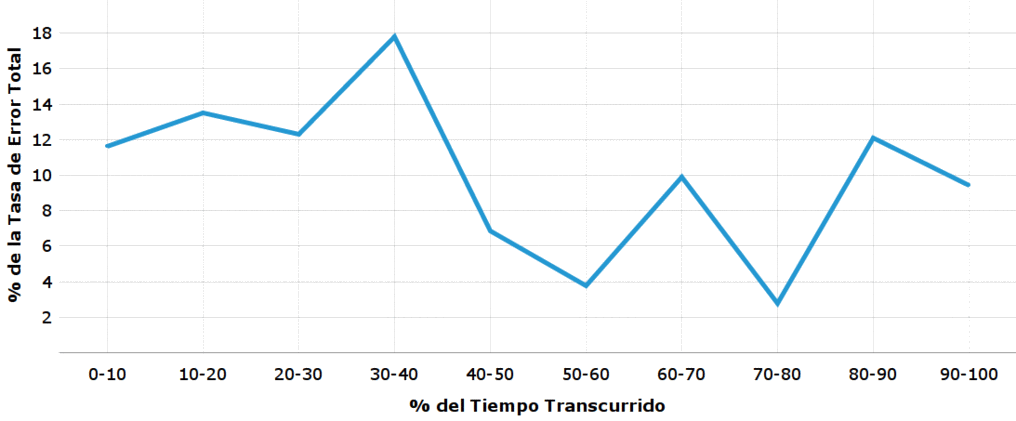
\includegraphics[width=1\linewidth]{./graphics/error_tiempo.png}
\caption{Distribuci\'on del error humano por etapas de la sesi\'on.}
\label{figure:gerror-tiempo}
\end{figure}
\end{columns}

\end{frame}

\begin{frame}{Resultados Obtenidos (6/7)}
\framesubtitle{Encuesta}
\begin{columns}
\column{0.35\linewidth}
\begin{table}[H] 
\centering
\tiny
\begin{tabular}{|r|r|r|r|r|}
\hline
            & Promedio \\
\hline
Vocabulario    & 6,17 \\
Comandos    & 6,58 \\
Entrenamiento  & 6,25 \\
Interfaz por Voz & 5,83 \\
\hline
\end{tabular}
\caption{Resumen de la encuesta realizada.}
\label{sec:tabla-encuesta}
\end{table} 
\column{0.65\linewidth}
\begin{figure}[ht]
\centering
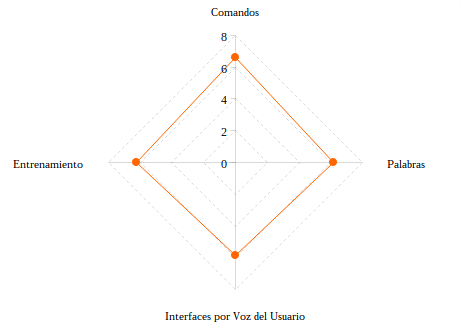
\includegraphics[width=1\linewidth]{./graphics/kiviat0.png}
\caption{Gr\'afico radial resumen de la encuesta realizada.}
\label{figure:kiviat-encuesta1}
\end{figure}
\end{columns}
\end{frame}

\begin{frame}{Resultados Obtenidos (7/7)}
\framesubtitle{Encuesta}

\begin{columns}
\column{0.35\linewidth}
\begin{equation*}
s_a=\frac{s-min_i}{max_i-min_i}
\end{equation*}

\begin{table}[H] 
\centering
\tiny
\begin{tabular}{|r|r|r|r|r|}
\hline
            & Promedio \\
\hline
Vocabulario    & 0,45 \\
Comandos    & 0,86 \\
Entrenamiento  & 0,55 \\
Interfaz por Voz & 0,5 \\
\hline
\end{tabular}
\caption{Resumen de la encuesta realizada. Valores reescalados.}
\label{sec:tabla-encuesta-normalizada}
\end{table}
\column{0.65\linewidth}
\begin{figure}[ht]
\centering
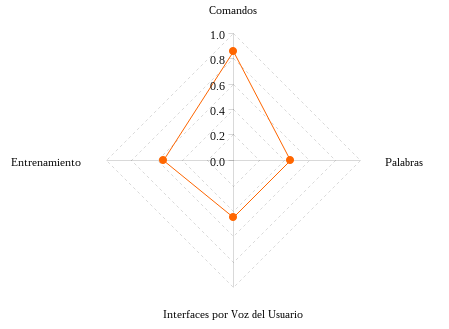
\includegraphics[width=1\linewidth]{./graphics/kiviat.png}
\caption{Gr\'afico radial resumen de la encuesta realizada. Valores reescalados.}
\label{figure:kiviat-encuesta2}
\end{figure}
\end{columns}
\end{frame}